\begin{surferPage}[Куммер]{Квартика Куммера}
	Эдуард Куммер стал в 1875 г. первым, кто специально сформулировал вопрос о максимальном количестве сингулярностей на поверхности степени $d$ (обозначим его через $\mu(d)$), а точнее говоря для поверхностей $4$-й степени, т.е. квартик.

Он доказал, что $\mu(4)=16$, как следствие, детально изучил поверхности с этим свойством. Особенно красивое семейство таких поверхностей задано следующим уравнением: 
    \[\bigl(x^2+y^2+z^2-\mu^2\bigr)^2 - \lambda
    \,y_0\,y_1\,y_2\,y_3,\]
    где $\mu$ - свободный параметр, а
    $\lambda$ зависит от $\mu$. $y_i$ выбраны как грани правильного тетраэдра для того, чтобы поверхность была симметрична:
	{\footnotesize
	\begin{align*}
	y_0&=1-z-\sqrt{2}x, &y_1&=1-z+\sqrt{2}x\\
    y_2&=1+z+\sqrt{2}y, &y_3&=1+z-\sqrt{2}y.
	\end{align*}}
Хотя большинство членов этого семейства имеют ровно $16$ действительных сингулярностей, но всё же не все. 
  \begin{center}
    \hspace*{-0.2cm}
    \begin{tabular}{@{}c@{\,}c@{\,}c@{\,}c@{\,}c@{}}
      \begin{tabular}{@{}c@{}}
        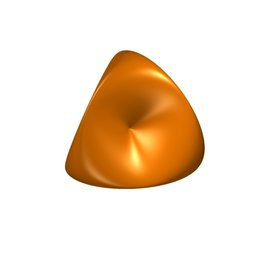
\includegraphics[height=1.4cm]{./../../common/images/kummer_0}
      \end{tabular}
      &
      \begin{tabular}{@{}c@{}}
        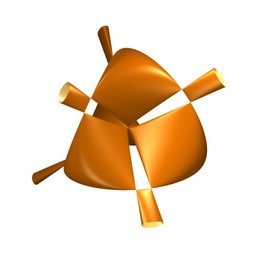
\includegraphics[height=1.4cm]{./../../common/images/kummer_1}
      \end{tabular}
      &
      \begin{tabular}{@{}c@{}}
        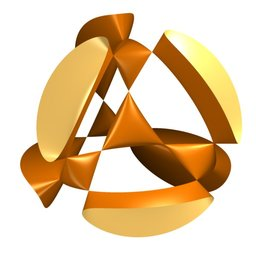
\includegraphics[height=1.4cm]{./../../common/images/kummer_2}
      \end{tabular}
      &
      \begin{tabular}{@{}c@{}}
        
\includegraphics[height=1.4cm]{./../../common/images/kummer_3}
      \end{tabular}
    \end{tabular}
  \end{center}
Для особых значений параметров несколько сингулярностей могут накладываться друг на друга.
\end{surferPage}
